Today I should be around for more talks. The day begins with a keynote!

\subsection{Keynote: Pierre-Yves Oudeyer on AI and Education}

{\bf Note:} Children are extraordinary learners! And typically do so without an engineer following them hand tuning every aspect of their learning algorithm and environment. \\

\begin{figure}[h!]
    \centering
    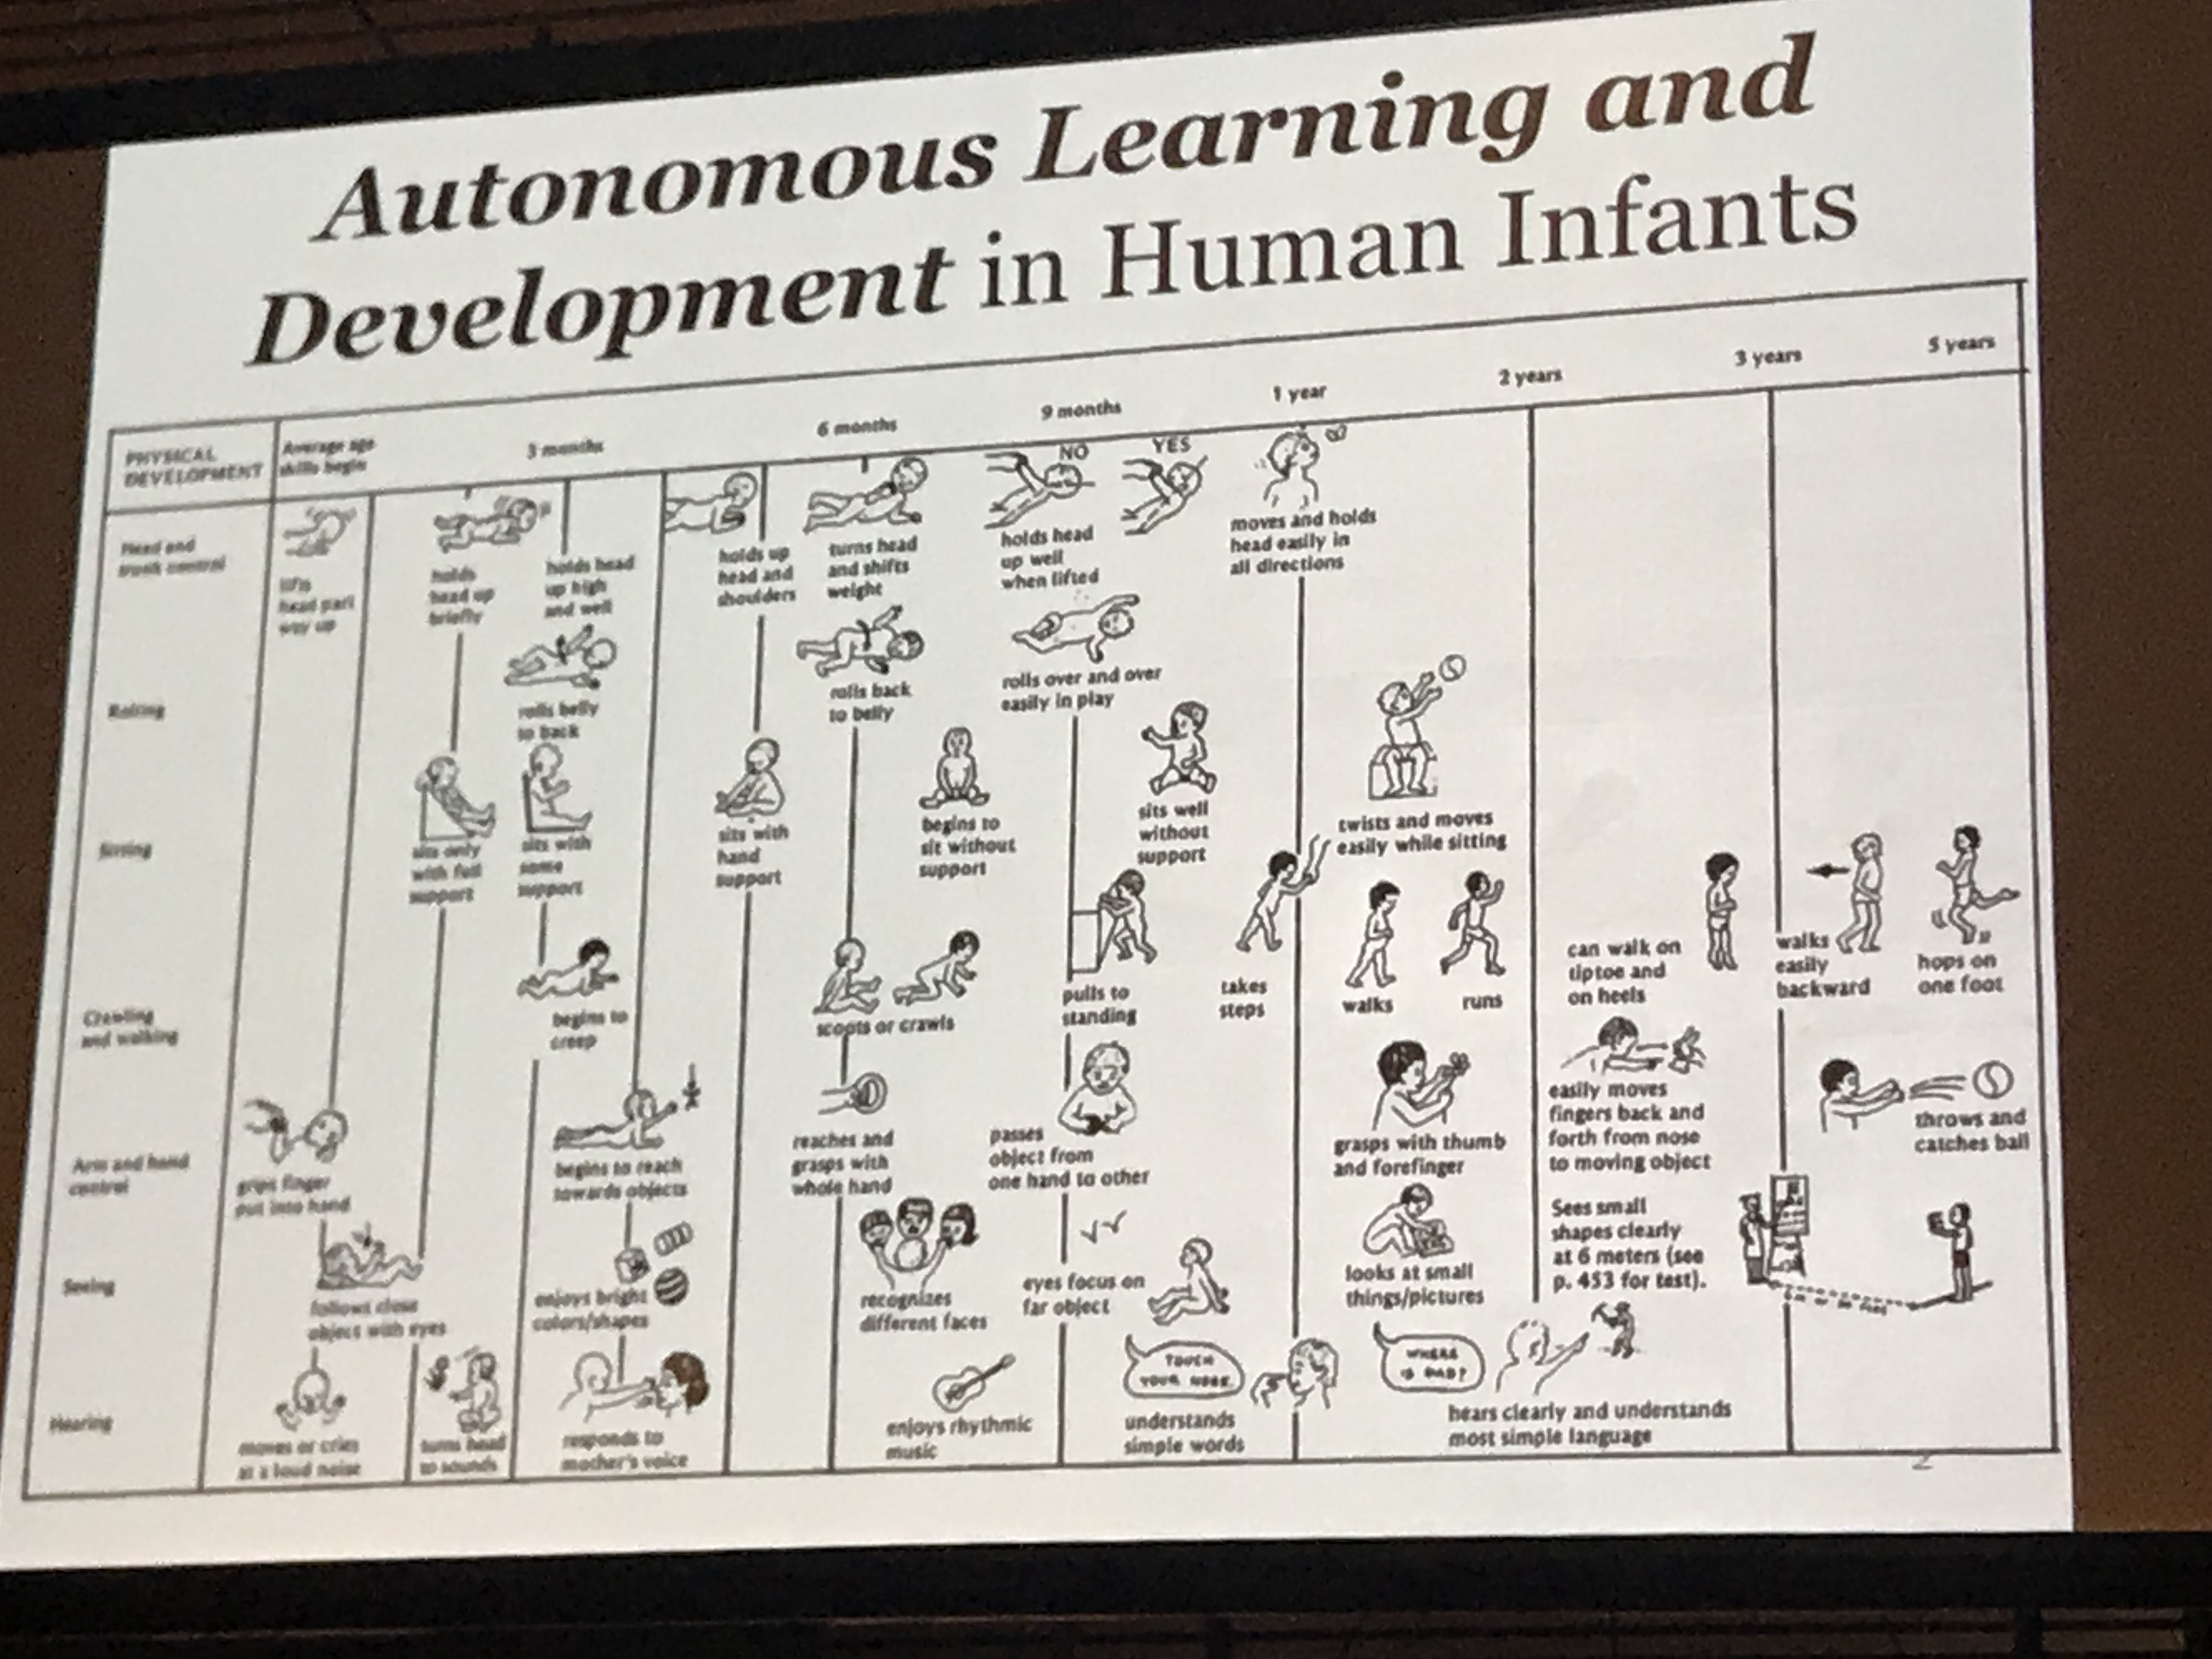
\includegraphics[width=0.4\textwidth]{images/child_learners.JPG}
    \caption{Learning and development in human infants.}
    \label{fig:child learners}
\end{figure}

Guiding Fields:
\begin{enumerate}
    \item {\it Cognitive Science:} Understanding human development and learning
    \item {\it Robotics:} new theory for lifelong and autonomous learning
    \item {\it Applications} in education technology.
\end{enumerate}


Example 1: study of {\it morphology}, body growth, and maturation in designing motor and perceptual primtives in a robot. \\

Example 2: consider language acquisition. Children learn new language very quickly. \\

Example 3: intrinsic motivation, play, and curiosity. \\

Q: How can we understand these practices, and harness them in AI tools, and build new educational tools around them? \\

\subsubsection{Intrinsic Motivation and Curiosity}

Consider {\it active exploration}: video of a baby playing with a variety of toys in a room over time (reminds me of the playroom domain from RL). \\

$\ra$ Similarly, give a baby a few toys, and a hollow cylinder suspended off the ground with a toy car inside of it. The baby over time tends to put the toy into the cylinder which knocks the car out of the tube (at which point the parent is very happy!). \\

$\ra$ But! When the car pops out of the tube, the baby also tends to pick up the car and put it back in the tube. \\

Other children experiment in very {\it different} ways; one kid picked up the block and hit the cylinder to make noises, and seemed very pleased by the noises. This was considered a ``failure" in the study, but was pretty sophisticated exploration! \\

{\bf Note:} Theories of intrinsic motivation, curiosity, and active learning drive to reduce uncertainty, experience novelty, surprise, or challenge. See~\citet{berlyne1960conflict} and~\citet{berlyne1978curiosity}. \\

{\bf Perspective:} The child is a sense making organism: explore to make good predictive models of the world and control it! \\

Q: Based on this perspective, what kind of modeling/algorithms are needed in order to explain these behaviors? \\

A: We use robotic playgrounds -- place robots in a playroom like environment, and encourage them to play to learn object models and affordances. Also place another robot in the playroom that gives ``feedback" (positive/negative reward) to play the role of a parent encouraging/discourgaing the baby.\\

Essential ingredients in these robots:
\begin{itemize}
    \item Dynamic movement primitives
    \item Object-based perceptual primitives (like infants, build on prior perceptual learning)
    \item Self supervised learning forward/inverse models with hindsight learning
    \item Curiositry-driven, self-motivated play and exploration.
\end{itemize}


\subsubsection{The Learning Progress Hypothesis}

Q: What is an {\it interesting} learning experiment for a robot/baby to conduct (to learn)? \\

Lots of answers in the literature: high predictability, high novelty, high uncertainty, knowledge gap, novelty, challenge, surprise, free energy, and so on. \\

{\bf This Work:} The Learning Progress Hypothesis~\cite{oudeyer2016intrinsic}:

\ddef{Learning Progress Hypothesis}{The ``interestingness" of an experiment is directly proportional to empirical learning progress (absolute value of derivative of the errors)}

$\ra$ Few assumptions on underlying learning machinery and on match between biases and real world. \\


{\bf Framework:} suppose we have some robots with motion primitives. Takes some sequence of actions to yield a trajectory:
\[
\tau = (s_t, a_t, s_{t+1}, \ldots).
\]
From this trajectory, the robot should learn, assuming some behavioral abstraction $\phi$:
\begin{enumerate}
    \item Forward model: $F_i : s, \theta \ra \phi_i$, with $\theta$ the parameters of the behavioral policy, $\pi_theta$.
    \item Inverse model: $I_i : s, \phi_i \ra \argmin_\theta ||\phi_i - F_i(s,\theta)||$
\end{enumerate}

Use these two models to measure ``competence progress" as a proxy of the empirical learning progress. \\

$\ra$ Example 1: hierarchical multi-armed bandits. Split a space into subregions, where an agent monitors the errors of each subregion. Use these errors to measure the learning progress over time. Then, in the bandit setting, can explore based on the ratio of these errors over time. \\

$\ra$ Example 2: explore omni-directional locomotion. Look at diversity (in terms of spread of states reached in some space) of outcomes by different exploration policies on a robot. Finding: curiosity-driven exploration is less-efficient than goal exploration.\\

Q: Why is curiosity driven exploration less efficient? \\

A: Forward model exploration (curiosity): knowing many ways to produce a few effects, inverse model exploration (goal): knowing a few ways to produce many effects. \\

Example: curiosity-driven discovery of tool use. Videos of a few robots playing with different tools (a robot with a cup learning to interact with a ball, a gripper robot learning to interact with a joystick). \\

$\ra$ Point: focus on playing with and manipulating objects in the world. The gripper robot learns to manipulate the joysticks, which moves the robot that can pickup the ball. Torso eventually learns to make a light, play a sound, and hide the ball in the cup. \\

Project: ``MUGL: exploring learned modular goal spaces"~\cite{laversanne2018curiosity}. Main idea is to extend these exploration techniques to high dimensional input (the robot examples above used a feature vector, not images). \\

$\ra$ MUGL can be used to discovery independently controllable features (learn to control a ball, and so on).

\subsubsection{Models of Child Development Data}

Experiment: modeling vocal development. Use exact same algorithms from before. \\

$\ra$ Goal: make experiments for the infant using the learning progress idea from before. \\

{\bf Finding:} Some self-organization of developmental structure in infants. First vocal track is learned (unarticulated sounds) and then learns articulated sounds. \\

$\ra$ Observe: regularities that tend to occur at the same time across different individuals, but some things change dramatically. Interactions between learning system and body morphology is stochastic, contingency in exploration, surprising that many things remain constant. \\

\begin{figure}[h!]
    \centering
    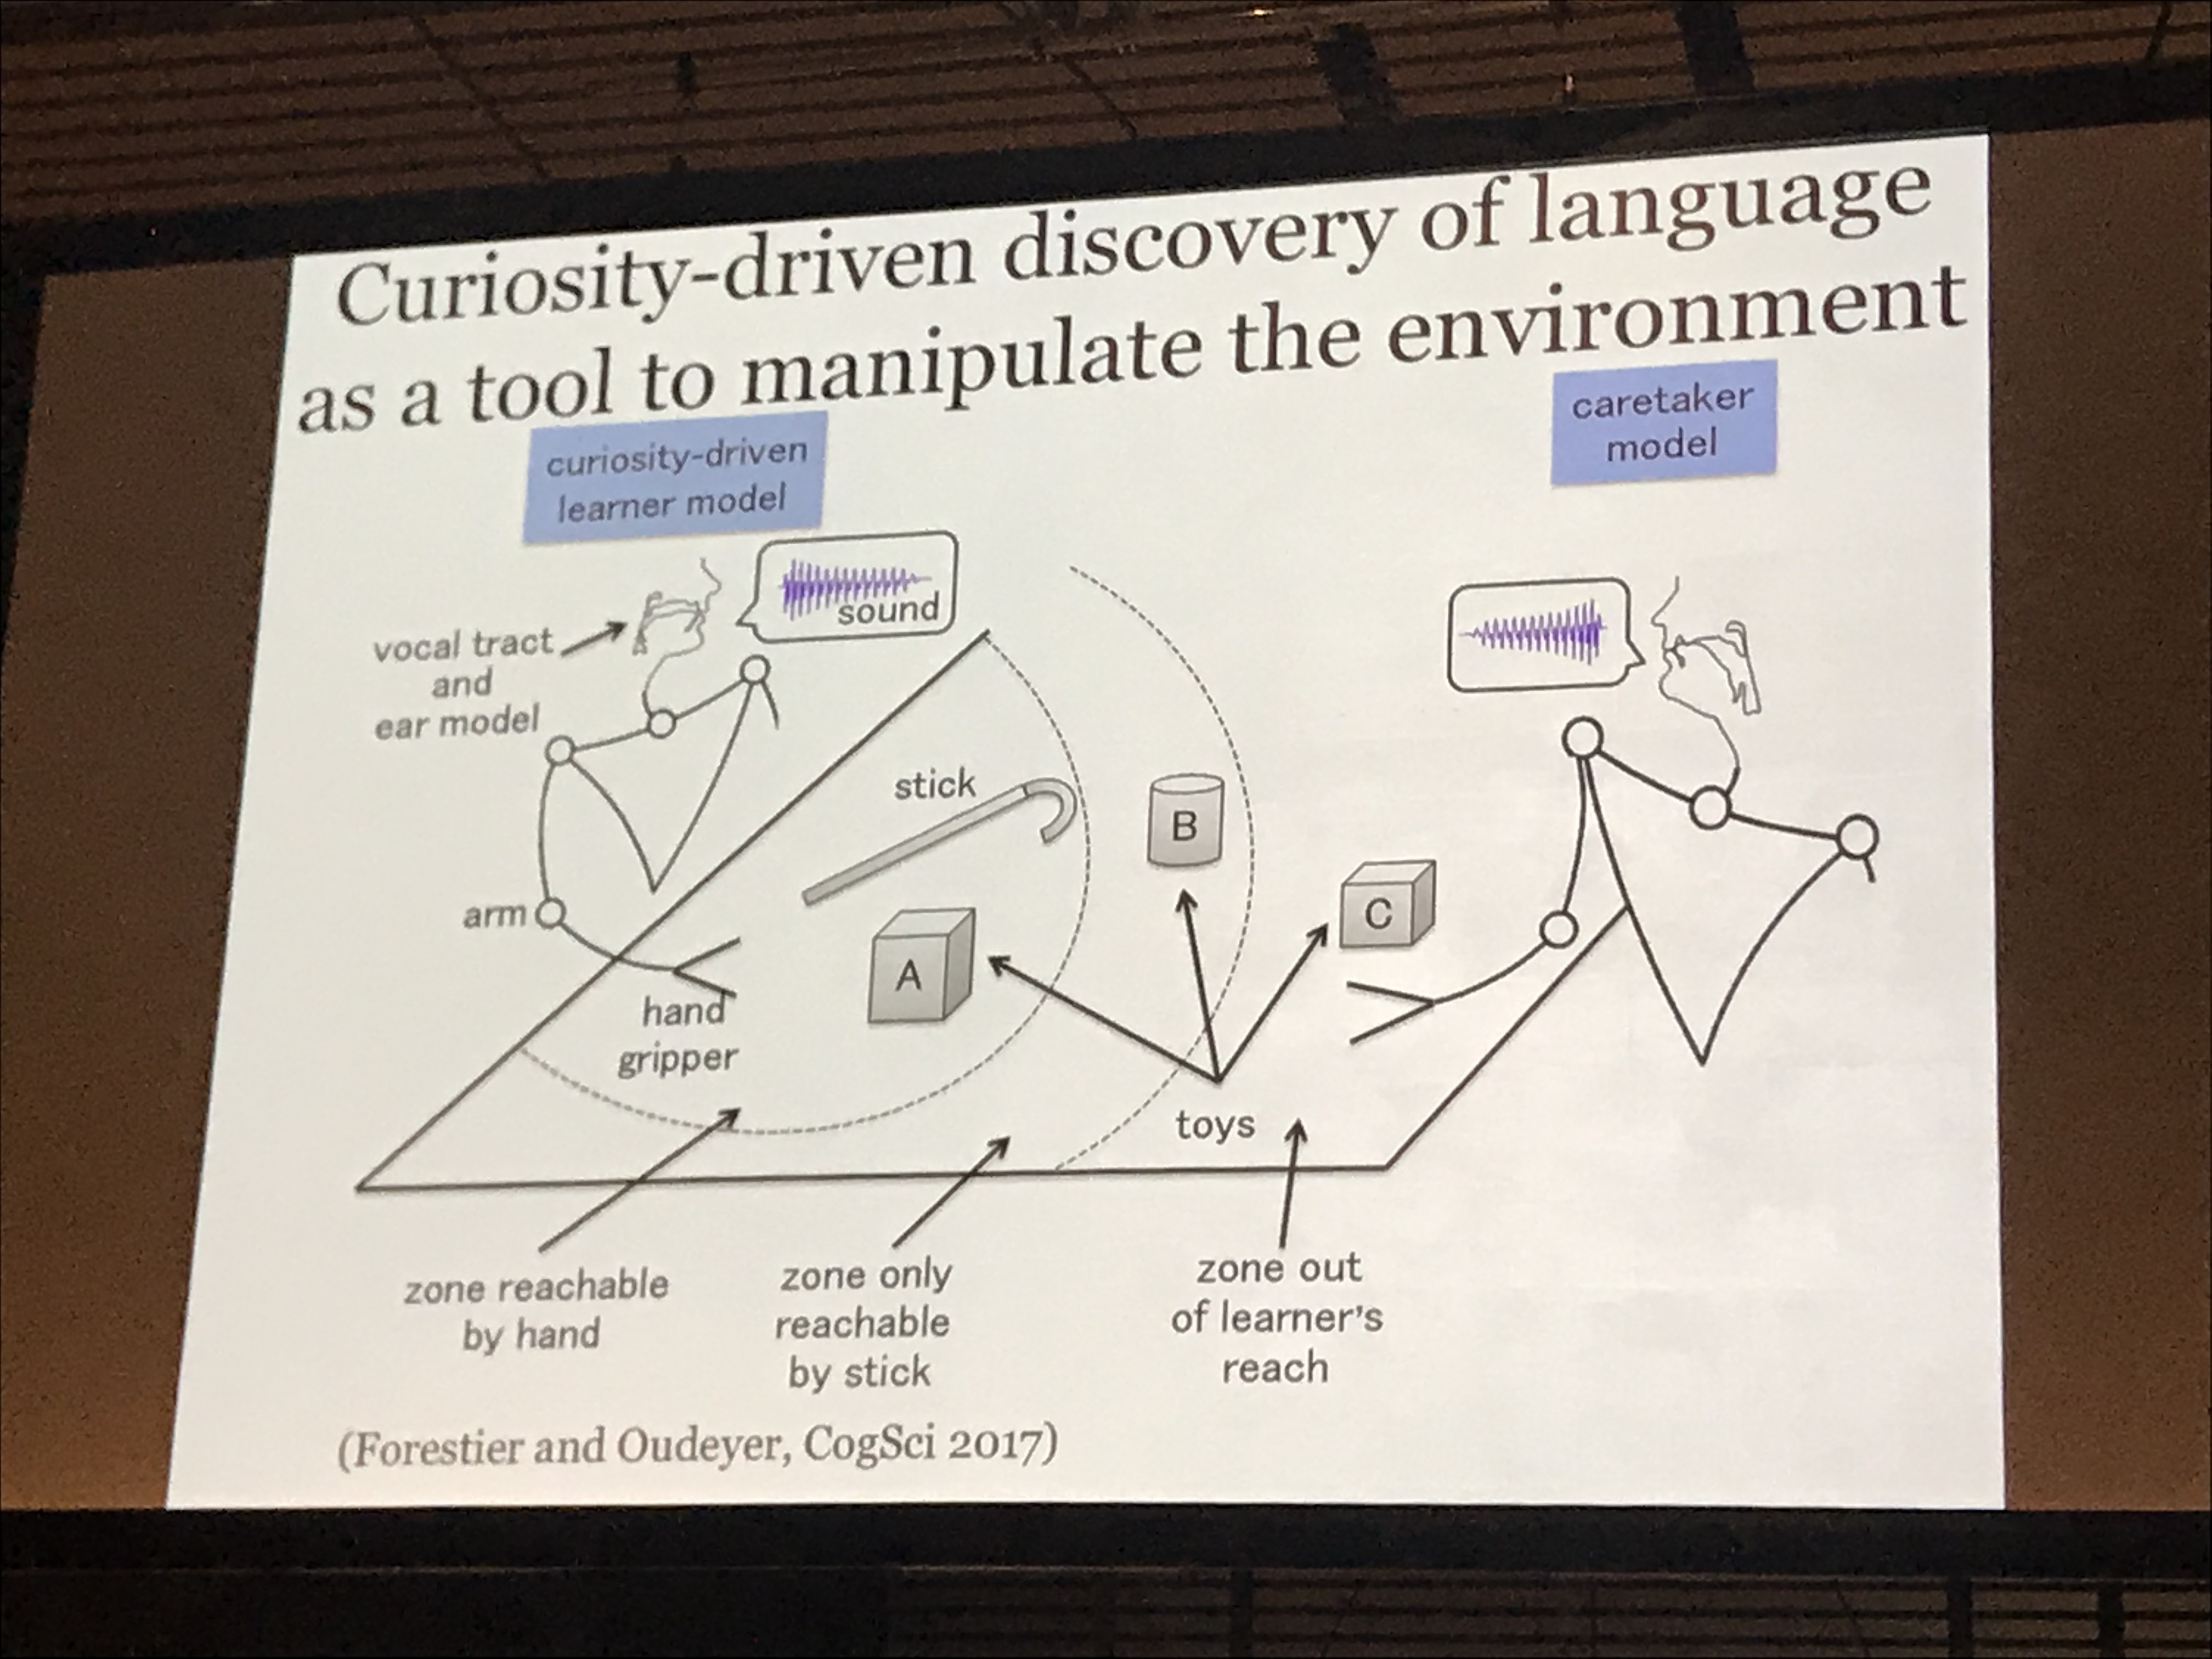
\includegraphics[width=0.4\textwidth]{images/curious.JPG}
    \caption{Curiosity-driven discovery of language}
    \label{fig:curiosity}
\end{figure}

The ``Ergo-Robots" (with Mikhail Gromov and David Lynch, I think?) \dnote{Lynch! :o}. Surreal video of robots learning to speak and interact with their environment and companions, see a sample video here: \url{https://www.youtube.com/watch?v=J0gM5i091JQ}. Robots learn to use language in a meaningful way through exploration. \\

$\ra$ Use similar ideas to come up with a realistic models of learning to use a vocal track. See: {\it Self-Organization in the Evolution of Speech}~\cite{oudeyer2006self}. \\

{\bf Finding:} The distributions of vowels we find in the world languages matches those of the systems that emerge in these curiosity-driven learning systems. This might explain some regularities of language structure. \\




Q: How is spontaneous exploration structured during free play? \\

A: Experiment! Let subjects play a bunch of games/tasks, with no guidelines. Just do whatever you want (play games like guitar hero, free to pick any level/song). \\

$\ra$ People tend to focus on levels of intermediate complexity; exploration follows a controlled growth in complexity, actively controlled by individuals' predictive models. 


\subsubsection{Applications in Educational Technologies}


{\bf Goal:} Develop technologies for fostering efficient learning and intrinsic motivation. \\

$\ra$ Project: KidLearn -- allows personalization of intelligent tutoring systems, based on experiments with $>$ 1000 children in 30+ schools. \\

Principle: graph (usually a DAG) defines difficulty of task/exercise type. This allows the system to sample exercises in some sequence (but still give the kids some choice among nodes in the graph). \\

Main study:
\begin{itemize}
    \item Examine learning impact based on these interventions.
    \item Compare to typical pedagogical expert (vs. their system).
    \item Find that students tend to achieve higher success rate with certain variations of the algorithm.
\end{itemize}

{\bf Takeaways:} Fundamental role of spontenous developmental exploration, can be harnessed to develop human-like robots and empower the learning process.

\subsection{Contributed Talks}
Next up some contributed talks.

\subsubsection{Devon Hjelm on Deep InfoMax~\cite{hjelm2018learning}}

{\bf Broad Goal:} Learn unsupervised image representations. \\

Example: video of a dog catching a snowball. What annotations make sense? (``Cute dog!", ``Good boy!"). \\

$\ra$ Not clear these are the right/useful annotations. \\

{\bf Point:} Don't always want supervised learning of representations. Annotations rarely tell the whole story, real world doesn't come with labels, and really want to find the underlying structure (annotations might not enhance this part). \\

Preliminaries:
\begin{itemize}
    \item Encoder: $E_\psi : \mc{X} \ra Y$, with $Y$ a representation.
    
    \item Mutul info; $I(X;Y) = D_{KL}(P(X,Y) \mid \mid P(x) p(y)$
\end{itemize}

$\ra$ Introduce amutual information estimator: encode an image into a representation. Take pairs of representations from images that aren't associated with each other, and treat these as {\it negative} samples,. \\

{\bf Approach:} 
\begin{enumerate}
    \item Encode input $X$ input $Y$ via $E_\psi$.
    \item Use output to estimate $\hat{I}(X;Y)$, and maximize this estimate.
    \item Just doing this alone isn't quite enough.
    
    {\it Intuition:} you might not pick up on the relevant locations of an image. Consider a picture of a cat, the background isn't as crucial as the information in the front.
    
    \item So: instead of maximizing the mutual info globally, instead maximize it {\it locally}. Perform this estimation/maximization across all locations simultaneously. See Figure~\ref{fig:cat}
    \item This yields local feature vectors for different regions of the image, which can then be stitched together into a global feature vector.
\end{enumerate}

\begin{figure}
    \centering
    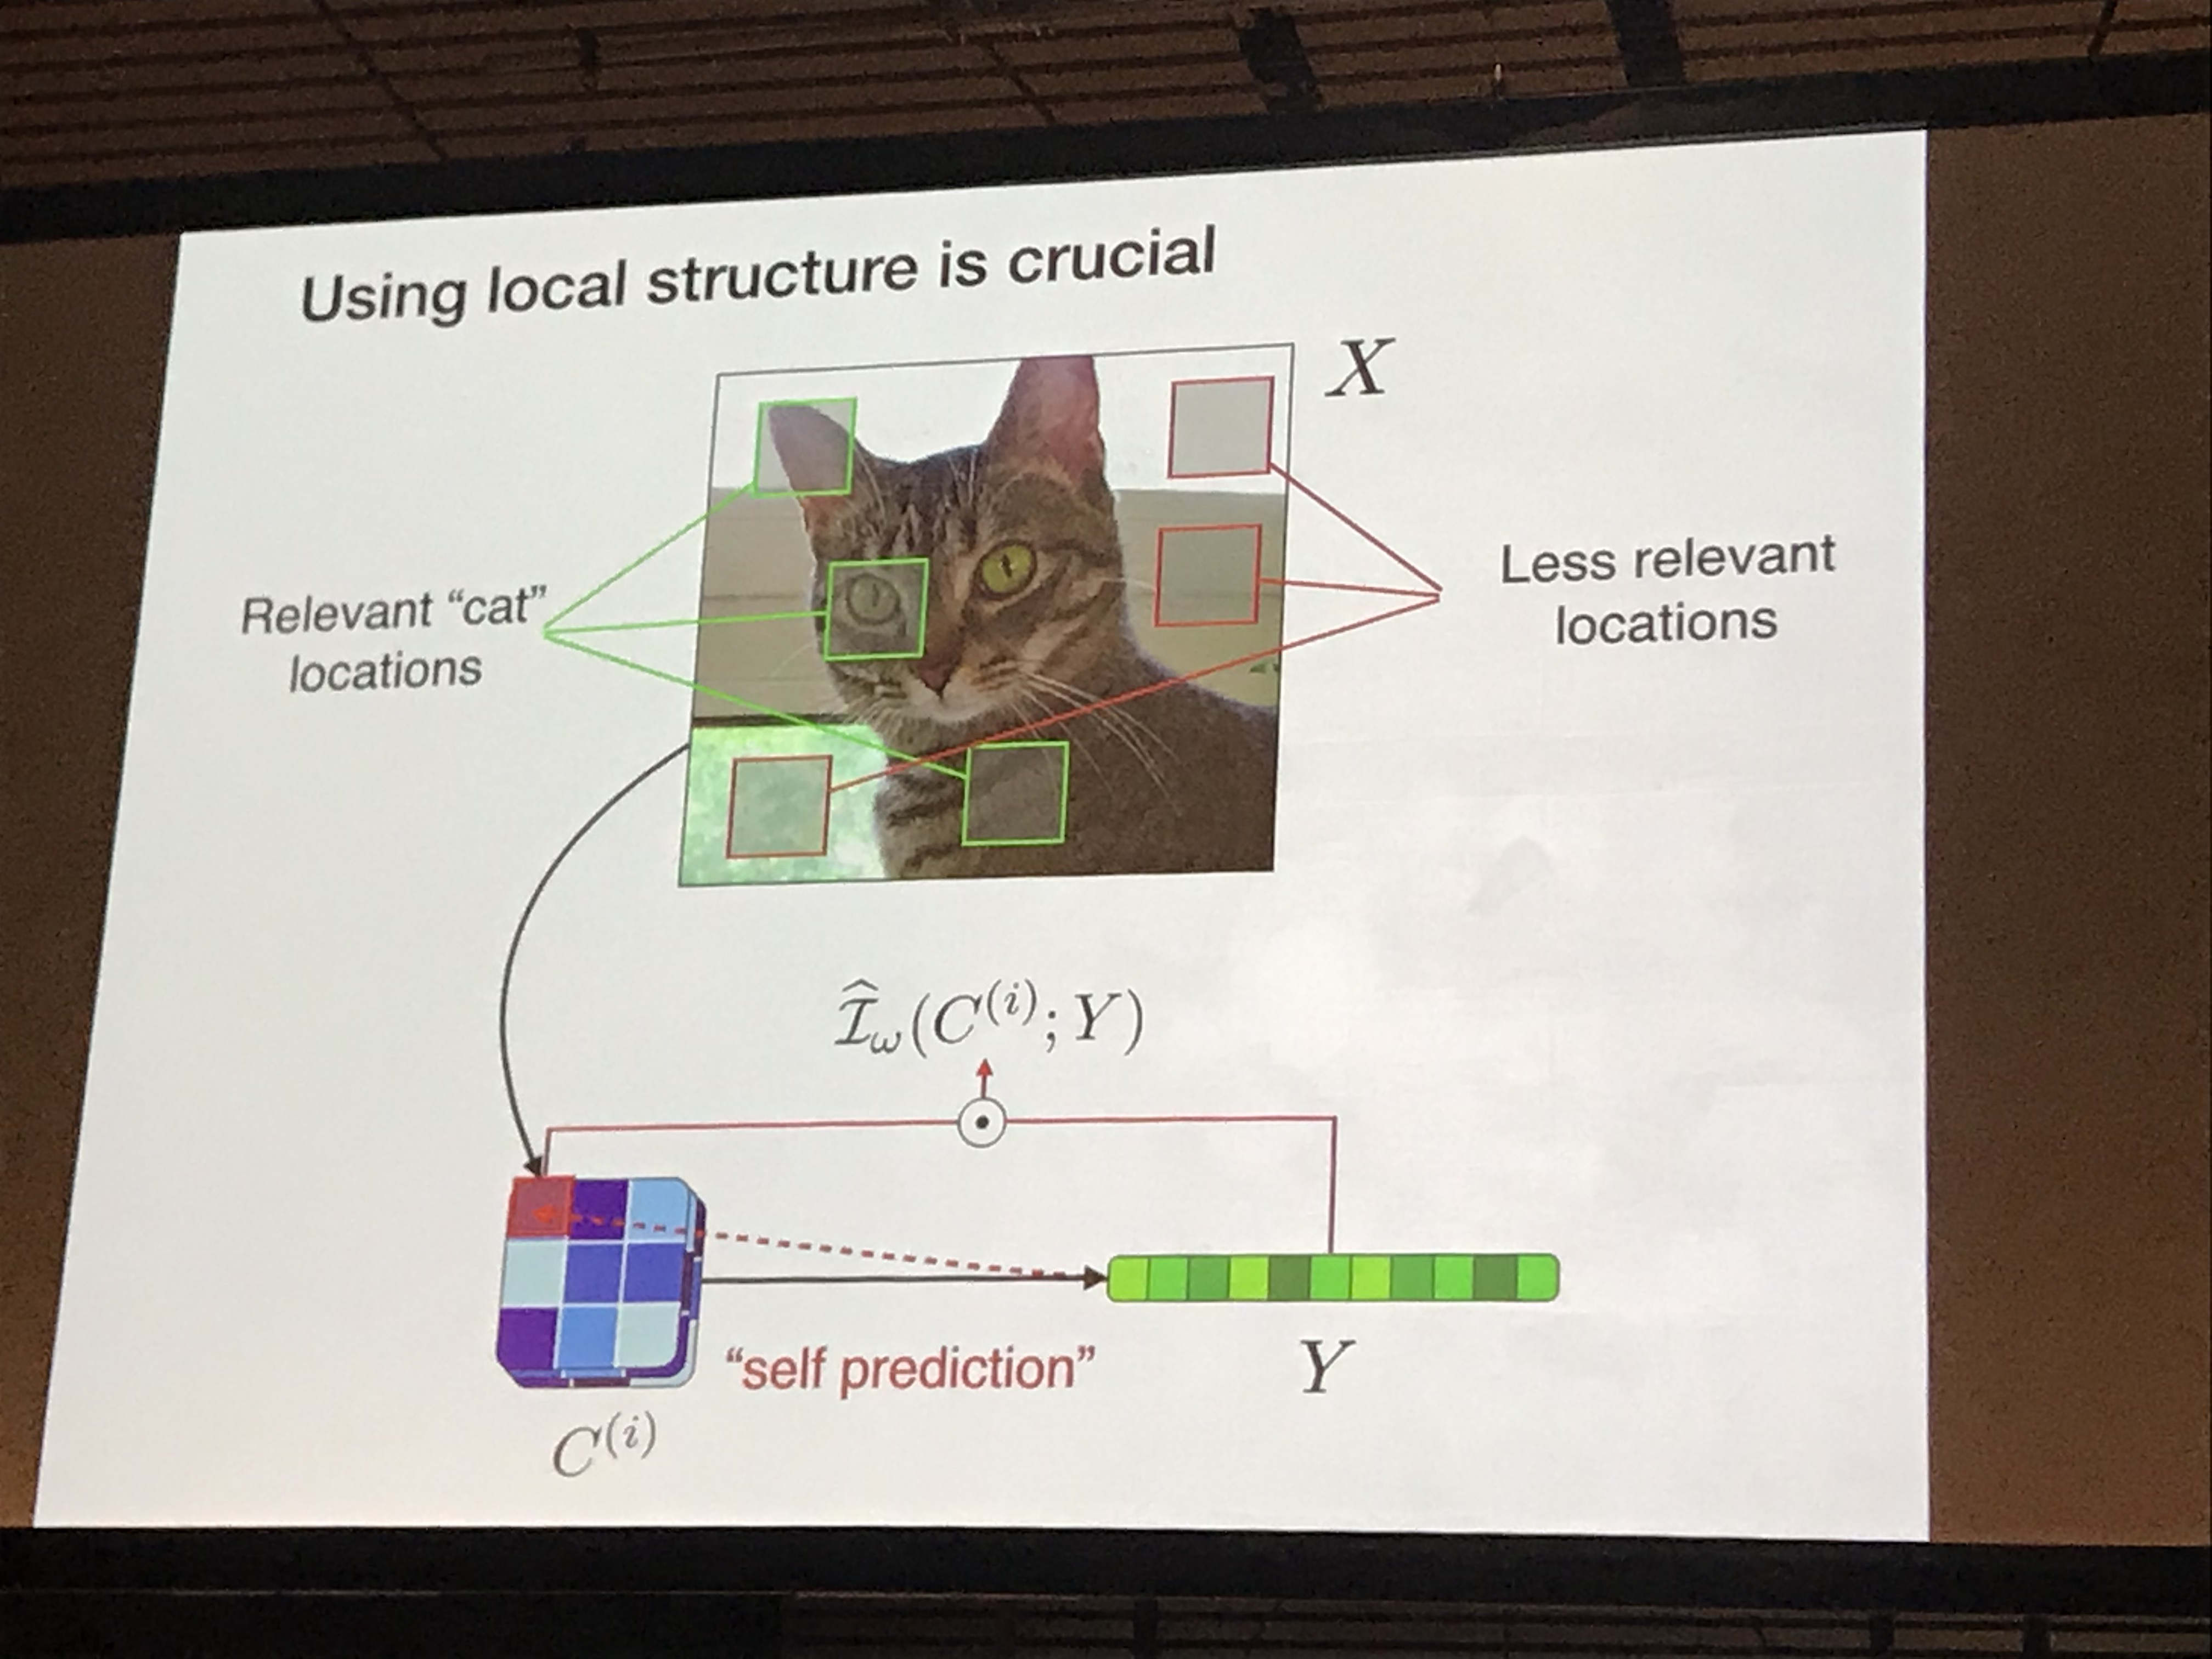
\includegraphics[width=0.4\textwidth]{images/cat.JPG}
    \caption{Extracing local feature maps via local mutual info estimation and maximization}
    \label{fig:cat}
\end{figure}

Evaluation: depends heavily on downstream task. Can measure mutual info, down stream performance on classification/regression tasks, and so on. \\

$\ra$ Deep Info Max performs very well when the learned representation is used in downstream tasks like classification. \\

Other tasks investigated: prior matching, coordinate prediction, relative coordinate prediction \\

\dnote{Off to more meetings.}